%!TEX root = main.tex

The methodology scheme is shown in Figure.\ref{fig.method}. 
%
During training stage, the training images are preprocessed using data augmentation techniques to increase the data diversity.  The augmented data are fed into deep convolutional neural network(ConvNet) for training. After deep ConvNet training is finished, it serves as a feature extractor and extracts deep features representing all training images. These deep features are used in the final step to train a support vector machine (SVM) for classification.
%
During the testing stage, the testing images are fed into the deep ConvNet for deep features extraction. These intermediate deep features are used as testing samples and fed into the trained SVM. The output of SVM is the final prediction.


\begin{figure}[!ht]
	\begin{center}
		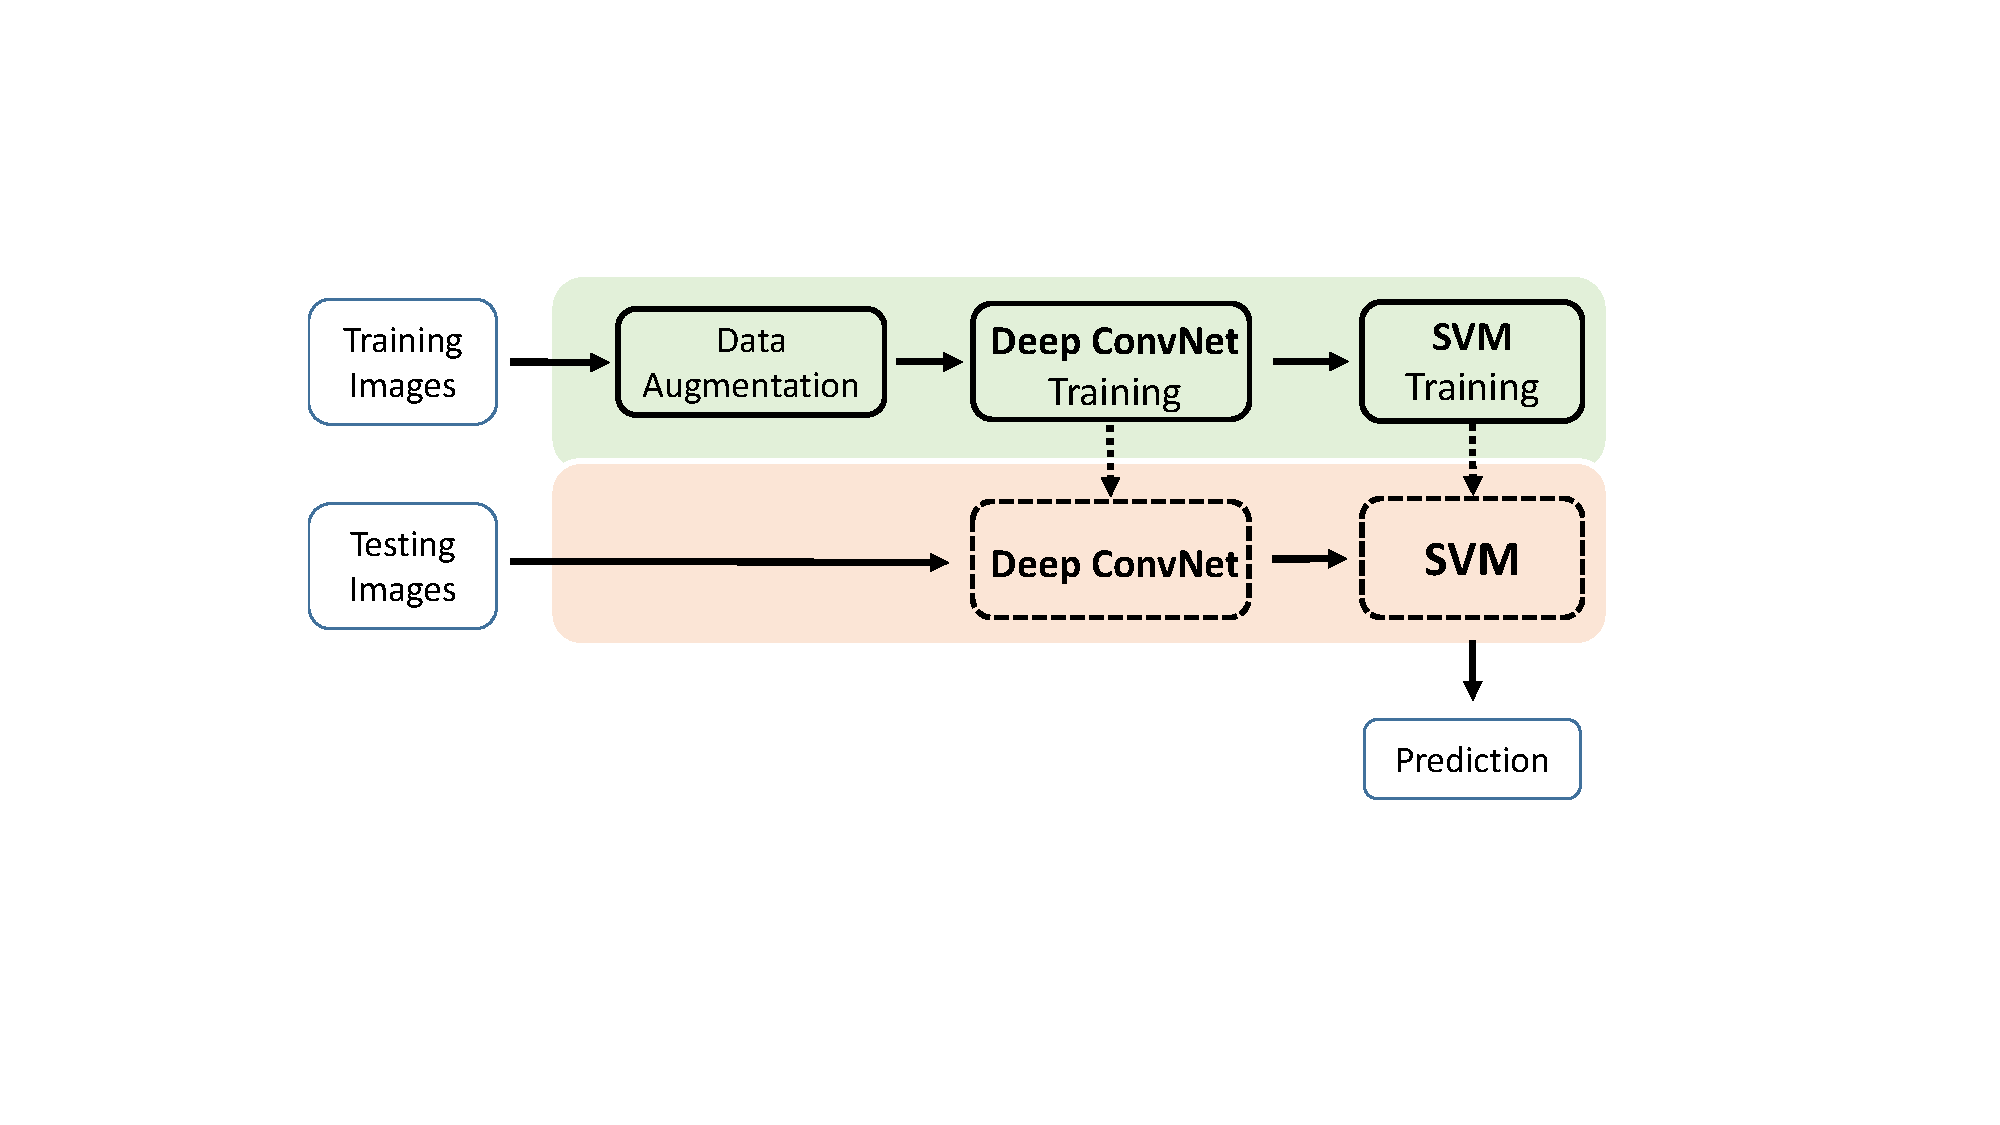
\includegraphics[scale=0.38,clip=true,trim = 50mm 55mm 28mm 50mm]{fig/figs/method_overview.pdf}
	\end{center}
	\caption{Overview of proposed approach.} 
	\label{fig.method}
\end{figure}

\subsection{Deep ConvNet Architecture}
An overview of the network architecture is shown in Figure.\ref{fig.cnn_arch}. 

Our proposed network is based on deep residual network proposed by Kaiming He \textbf{et al.}\cite{he2016deep}. Deep residual  network has been proven to outperform other deep plain networks because it addresses the degradation problem by reformulating the layers as learning residual functions instead of learning unreferenced functions. 
%
Table\ref{tab.cnn_params} shows the details of our network. The input size of our deep ConvNet is $512\times512$ and the number of channels is $1$.
The first two layers of our network are convolutional layers which has 96 $7\times7$ filters and the stride is 2. The third layer has 64 $7\times7$ filters and the stride is 2. 
%
\textit{conv4}, \textit{conv5}, \textit{conv6} and \textit{conv7} are composed of residual building blocks. Specifically, there is a max pooling layer before  \textit{conv4}. The parameters inside the brackets specify the residual building block size. 
%
The multiplier after bracket specifies the multiplicity of the that block in that layer. More details can be seen in \cite{he2016deep}. 
%
The global pooling layer in \textit{conv8} generates $1\times1,2048$ output and the last layer uses 5 $1\times1$ filters to generate the final prediction. 
%
The number of parameters of proposed deep ConvNet is $24.26$ million. 
%
We use Relu\cite{nair2010rectified} as intermediate activation function.
%

The novelty of our network is that we use $512\times512$ as network input size. The reason is that we preserve the detail of fingerprint as much as possible. Empirically we found the performance drop significantly when resizing the fingerprint samples to $224\times224$. 
%
\begin{figure}[!ht]
	\begin{center}
		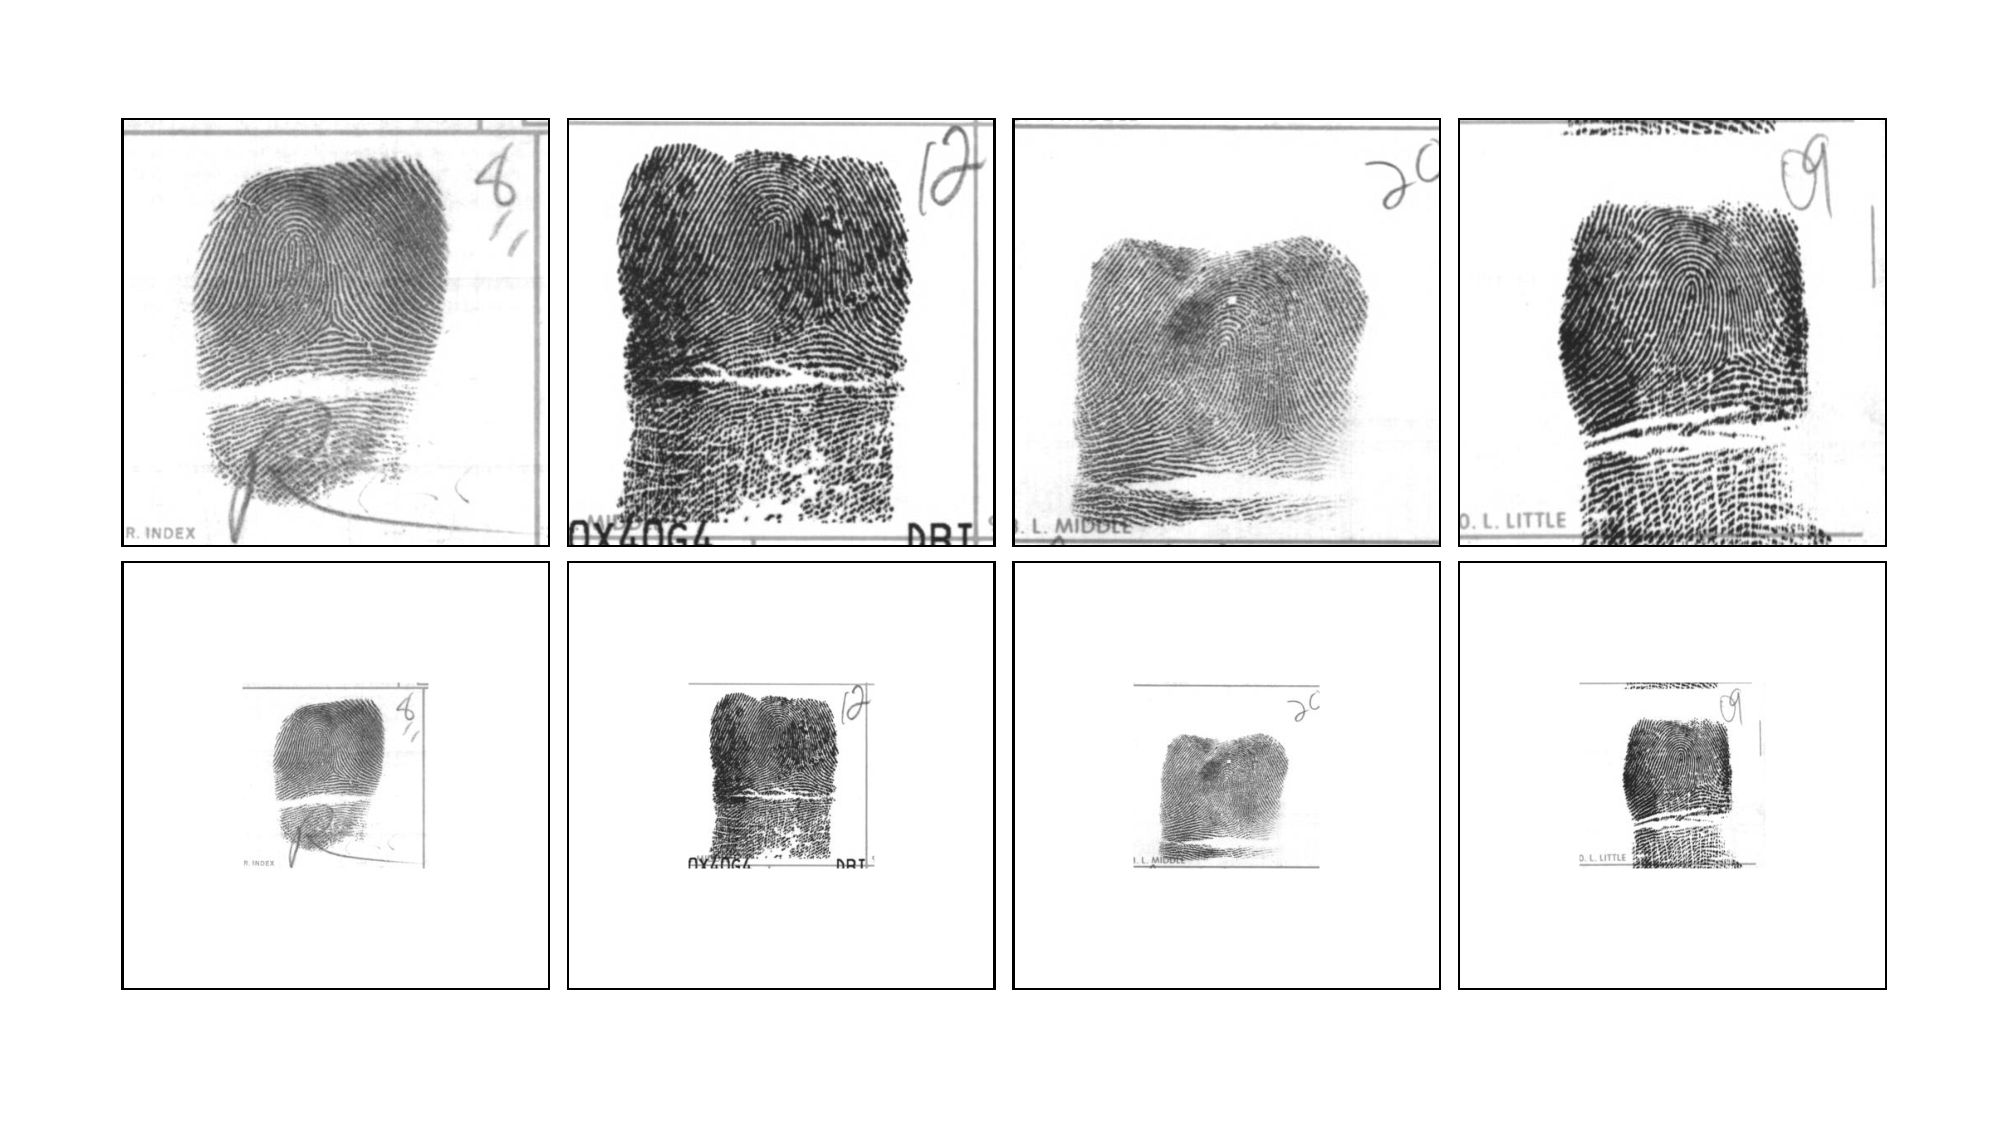
\includegraphics[scale=0.28,clip=true,trim = 20mm 15mm 10mm 10mm]{fig/figs/resize_examples.pdf}
	\end{center}
	\caption{NIST SD14 Images under different resolutions. The top row are images in $512\times512$ and the bottom row are images in $224\times224$. Ridges of top images are more distinguishable than that of bottom images. } 
	\label{fig.resize_examples}
\end{figure}

As shown in Figure\ref{fig.resize_examples}, after down-sampling the images to $224\times224$, the fingerprints are blurred, leading to the loss of important information such as deltas and cores.
%
There are basically two solutions. The first one is to localize the fingerprint in the image and crop out a specific smaller region that mostly contains the fingerprint. This approach relies on the localization accuracy which maybe a bottleneck.
%
Another solution is to maintain the original solution of the fingerprint. However, this solution will result in huge computational cost and high memory usage when training.
%
We adopt the second solution. After carefully looking at the fingerprint samples under different resolutions, we decide to use $512\times512$ as input size for two reasons. First, it is the original image size of NIST SD4. Second, resizing original NIST SD14 images to this resolution can preserve sufficient details for classification.
%
To reduce the computational cost, we add \textit{conv1} and \textit{conv2} with stride 2 to down-sample the input images. As we can see in Table.\ref{tab.cnn_params}, after \textit{conv2}, the feature map size is $128\times128, 96$. The spatial size is reduced (from$512 \times 512$ to $128 \times 128$) and spatial information is stored in the increased channels (from $1$ to $96$).

\begin{figure*}[!ht]
	\begin{center}
		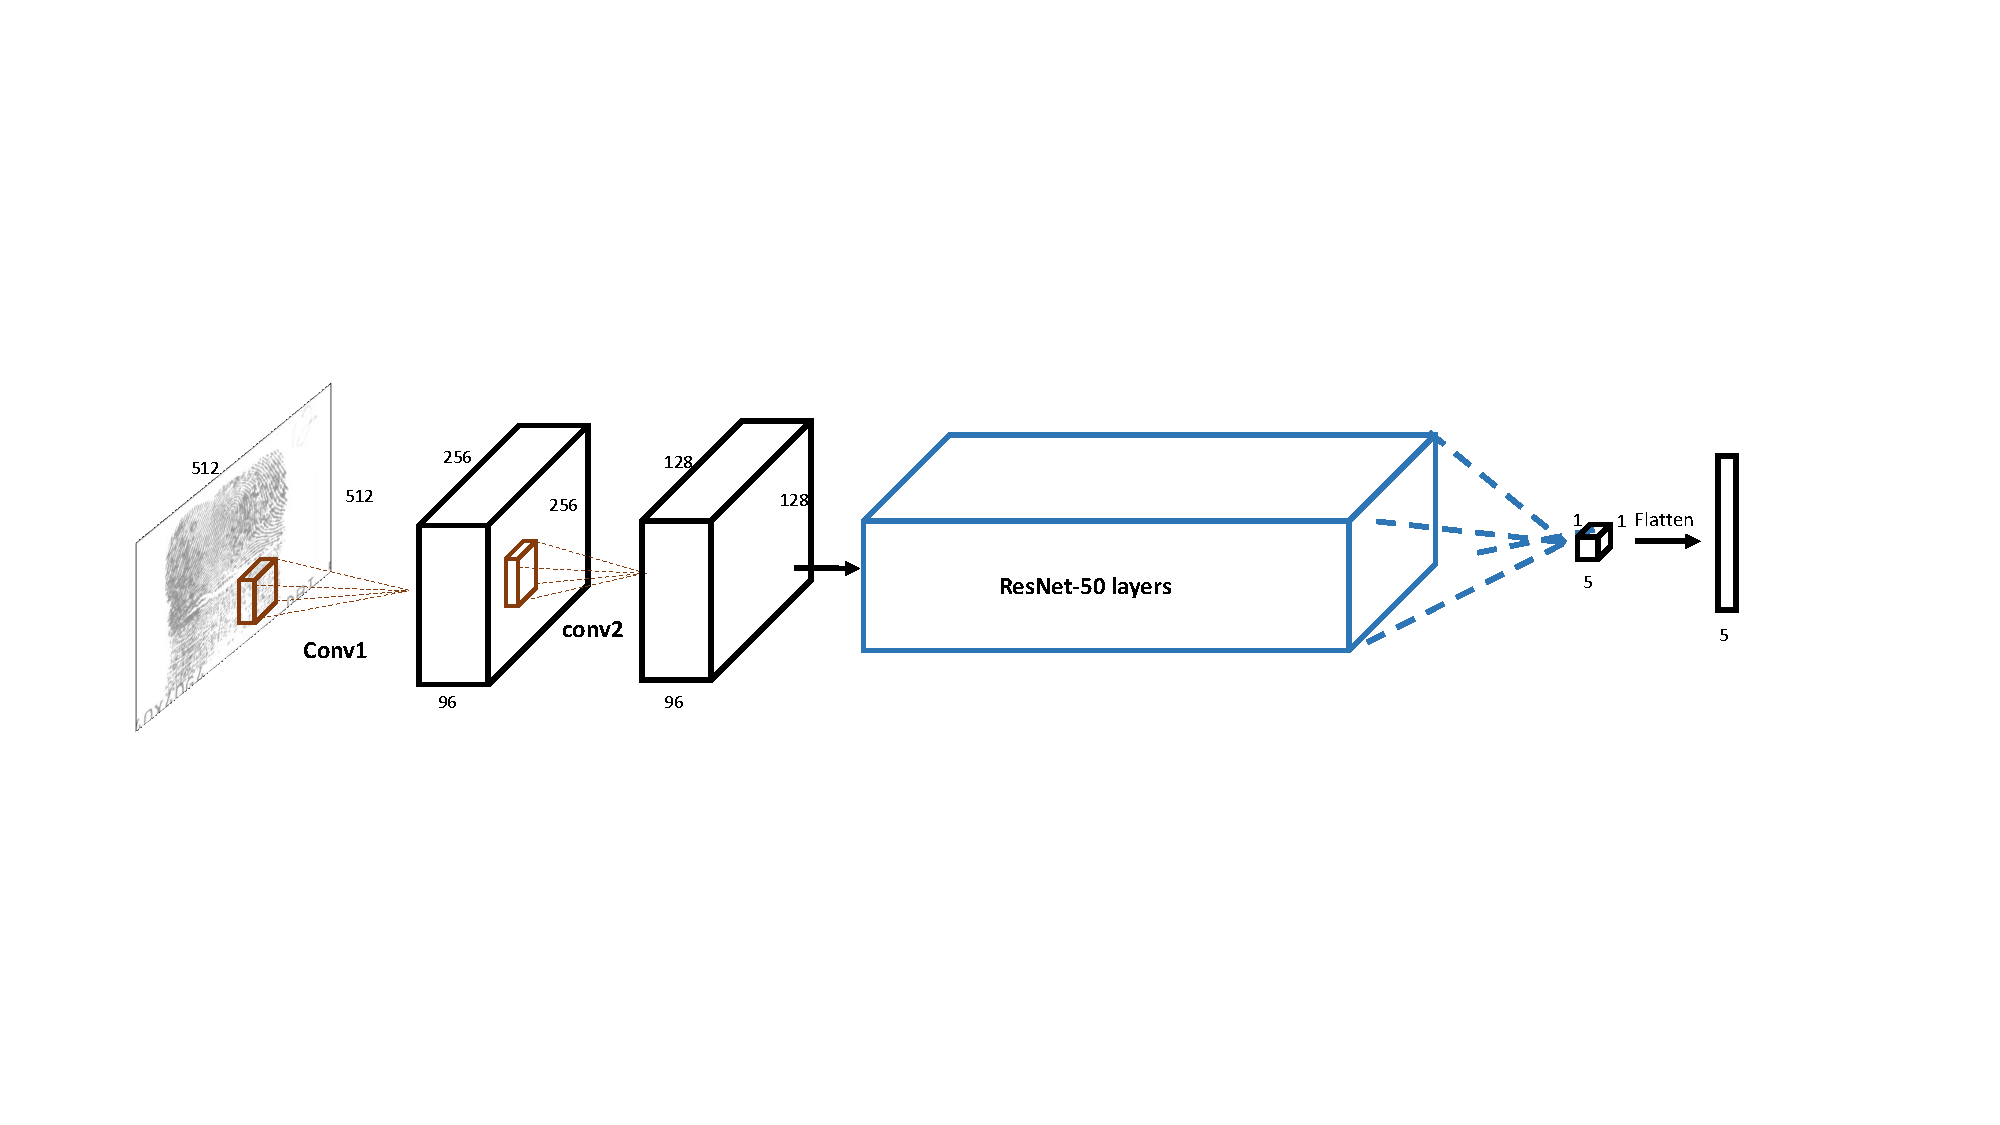
\includegraphics[scale=0.65,clip=true,trim = 20mm 65mm 30mm 65mm]{fig/figs/cnn_arch.pdf}
	\end{center}
	\caption{Architecture of proposed CNN.} 
	\label{fig.cnn_arch}
\end{figure*}


\begin{table}[!ht]
	\centering
	\caption{Detail of proposed deep ConvNet. The format is inspired by \cite{he2016deep}}
	\label{tab.cnn_params}
	\begin{tabular}{l}
		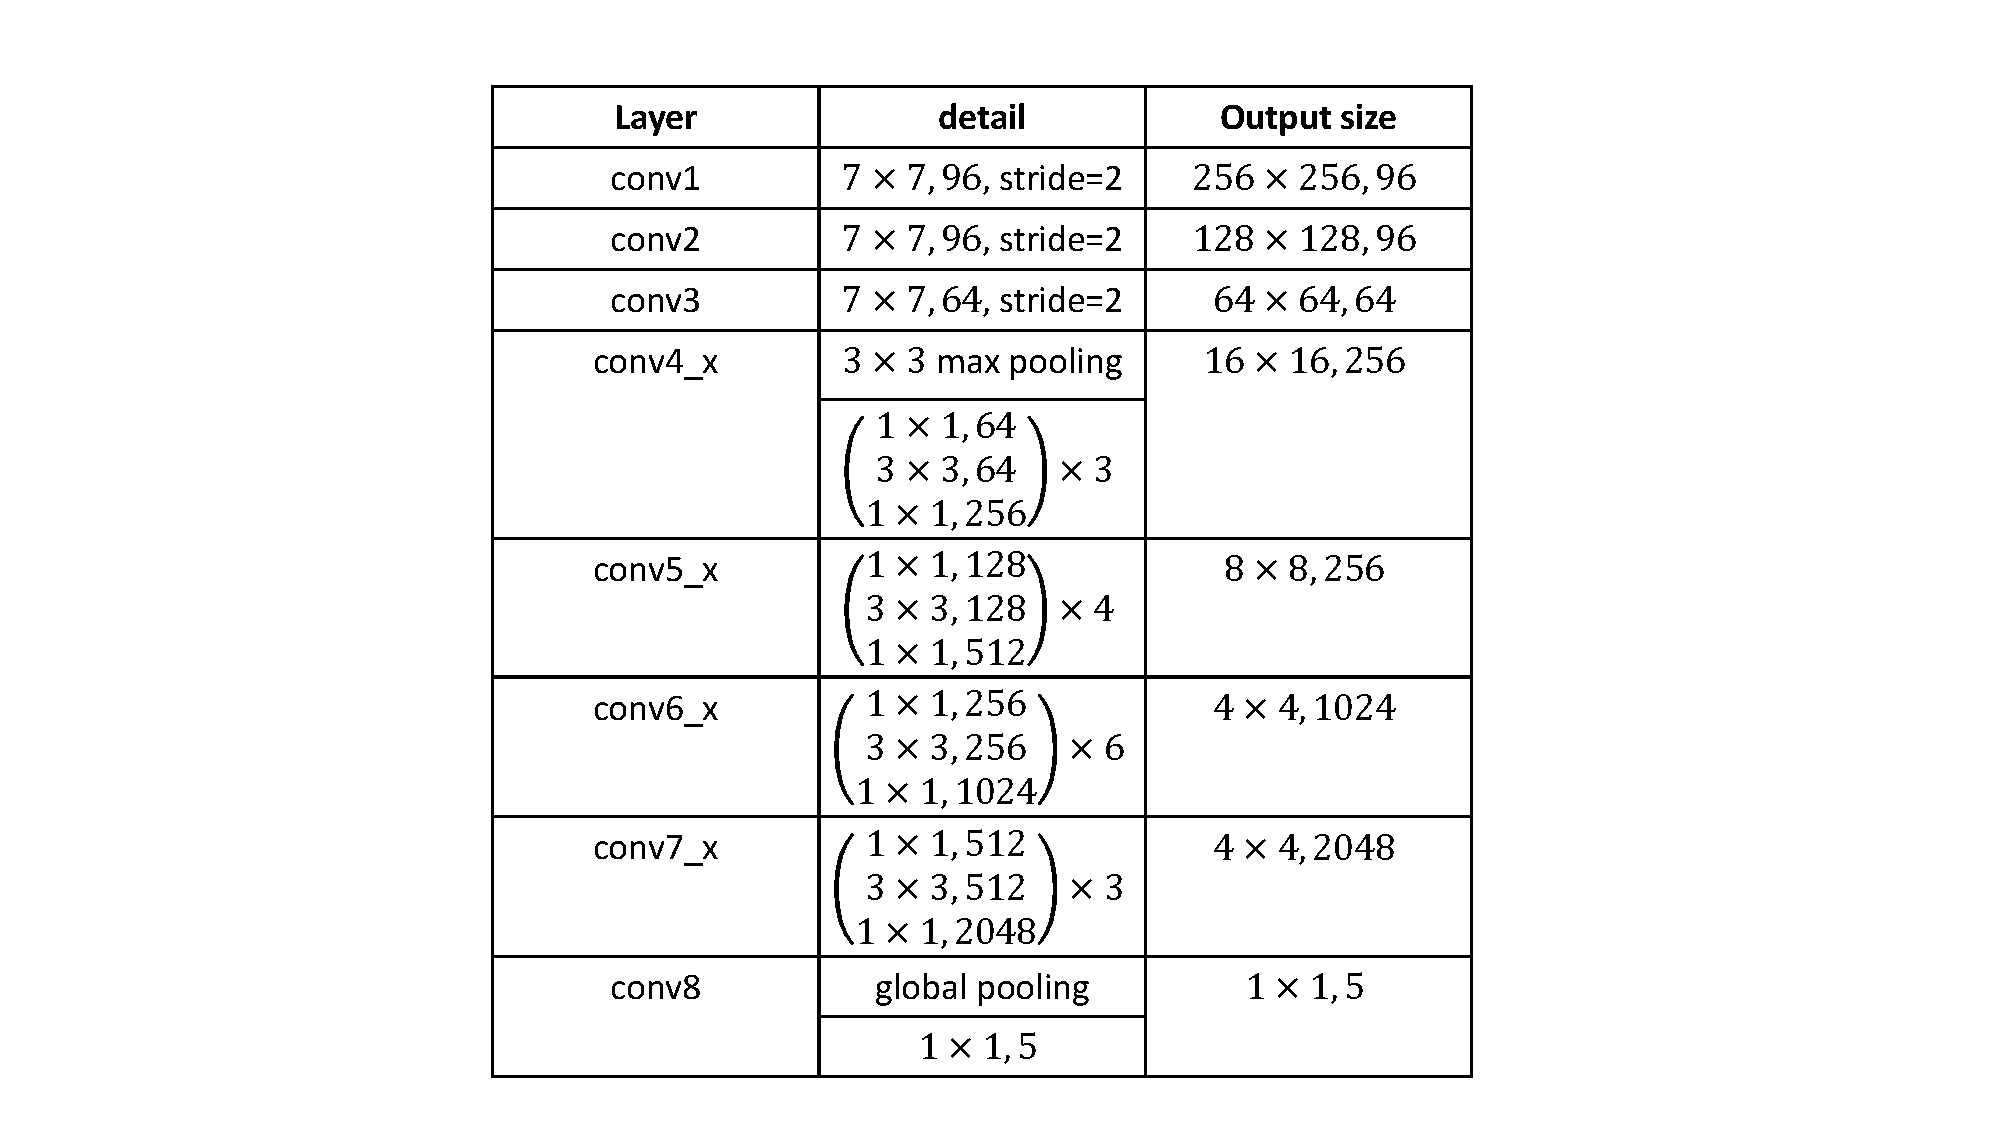
\includegraphics[scale=0.45,clip=true,trim = 78mm 5mm 70mm 5mm]{fig/figs/cnn_table.pdf}
	\end{tabular}
\end{table}


\subsection{Data Augmentation}
Due to the wild nature of the fingerprints samples, the fingerprints may exhibit a wide range differences in terms of position, rotation, brightness and contrast. To enhance the generalization ability of our ConvNet, we adopt data augmentation techniques to increase the data diversity.

During training stage, the input images will go through a augmentation process.
%
The data augmentation includes:
	
During training, we have applied three data augmentation techniques on segmented pill images to augment training dataset. 

\begin{enumerate}

	\item Random Cropping. The input images are first resized to $532 \times 532$. We randomly cropped a $512\times512$ region from the resized images.
	\item Random Rotation. We randomly rotate the input images by $\omega$ degrees where $\omega \sim uniform (-30\degree, 30\degree)$.
	\item Random Brightness.  Random brightness change is performed on the input images. The gray scale of the input images $I$ are change to $I + \delta$ where $\delta$ is  sampled from $uniform (-50, 50)$.
	\item Random Contrast. We randomly change the contrast of images. The contrast factor is sampled from $uniform (0.4, 1.6)$.

\end{enumerate}

\subsection{SVM}
The deep ConvNet only serves as a feature extractor and we use non-linear SVM as a classifier. The kernel is radial basis function(RBF). The gamma of RBF kernel  is set to be $\frac{1}{n}$ where $n$ is the feature dimensionality. The penalty for error term $C$ is set to be $1.0$. 
%
We use the output of  conv7\_x as features. As such, each sample is represented by a feature vector $x \in \mathbb{R}^d$ where $d=4*4*2048=32768$. The output of SVM is the predicted label $\hat{y} $ indicating one of the fingerprint classes.







